% \errorstopmode %  stop on error
\batchmode %  disable output generation
% preambolo per doppia compilazione HTML/PDF
\ifx\pdfoutput\undefined      % compilazione htlatex
\documentclass{article}
\DeclareGraphicsExtensions{.png, .gif, .jpg}

\else                         % compilazione pdflatex
\documentclass{article}

% packages
\usepackage{graphicx}
\usepackage{listings}
\usepackage{fancyhdr}
\usepackage{wrapfig}
\usepackage{multirow}
\usepackage{lscape}
\usepackage{amssymb,amsmath}
\usepackage[hyperindex]{hyperref}
\usepackage{caption}
\captionsetup{width=1.1\textwidth}
% caption font smaller
\captionsetup{font=small}

% page setup
\pdfpagewidth 8.5in
\pdfpageheight 11in
\setlength\textwidth{6.0in}
\setlength\textheight{8.1in}
\setlength\oddsidemargin{0in}
\setlength\evensidemargin{0in}
\setlength\topmargin{-0.6in}
\setlength\footskip{0.6in}
\setlength\headsep{0.6in}

% custom commands
\newcommand{\percent}{\,^0\!/_0}

%\newcommand{\href}[2]{\Link[#1]{}{} #2 \EndLink}
%\renewcommand{\hypertarget}[2]{\Link[]{}{#1} #2 \EndLink}
%\renewcommand{\hyperlink}[2]{\Link[]{#1}{} #2 \EndLink}

\hypersetup{
    pdfnewwindow=true,      % links in new window
    colorlinks=true,        % false: boxed links; true: colored links
    linkcolor=blue,          % color of internal links
    citecolor=magenta,      % color of links to bibliography
    urlcolor=blue           % color of external links
}
\fi


\begin{document}
\pagestyle{fancy}
\renewcommand{\sectionmark}[1]{\markright{\slshape \thesection\ #1}{}}


% author should reflect on the fancyfoot
\author{M. Ungaro, K. Joo}
\fancyhead[R]{\bf\rightmark}
\fancyhead[L]{e1-6 analysis}
\fancyfoot[R]{ \sl M. Ungaro, K. Joo}
\fancyfoot[L]{ \sl UCONN/JLAB}
\title{\large e1-6 Electron Identification}
\maketitle

\abstract{This chapter describes the electron identification for the e1-6 dataset.
The candidate electrons are all the negative time-based tracks that passed the hardware trigger.
The cuts are based on the candidate's reconstructed momentum and its signals on
the Electromagnetic Calorimeter and the \v Cerenkov counter.
When needed, the cuts are sector-dependent.}

\tableofcontents

\clearpage\newpage


\section{Electron identification}

In CLAS electro-production experiments
the scattered electron defines the timing of each event,
so it is particularly important to
make sure that their identification is correct and that
there is no contamination from particles such as $\pi^-$.

We consider {\it candidate electrons} every negative track
that produced a hardware trigger (this trigger condition is ensured by choosing
the first entry in the EVNT bank). The track is also required to have
hit matches in the CLAS \v Cerenkov (CC)\cite{bib:cc}, Drift Chambers (DC)\cite{bib:dc},
Electromagnetic Calorimeter (EC)\cite{bib:ec} and Time of Flight (SC or TOF)\cite{bib:ftof},
and to have time-based reconstruction (positive DC status word in DCPB).

Starting from a candidate electron, we use the following studies, detailed in the following sections,
to defined good electron:

\begin{itemize}
    \item CC $\theta$, $\phi$ and time matching in the detector
    \item EC Threshold
    \item EC Sampling Fraction
    \item Track Coordinates in the EC plane
    \item Minimum Ionizing Particles rejection in the EC
    \item Electromagnetic Shower Shape in the EC
    \item {\it Number of photo-electrons ($nphe$) in the CC
    This cut is not used anymore for identification,
        but the distributions will be shown for comparison with other analyses of e16 data }
\end{itemize}

For each individual cut we will show four histograms to illustrate its impact:

\begin{itemize}
    \item[a.] Variable distribution when no cut at all is applied.
    \item[b.] Variable distribution when all other pid cuts but this one are applied:
    this helps refining cut parameters.
    For example, when looking at the sampling fraction, applying all other
    cuts to helps clean up the plot and to better estimate the sampling fraction
    cut. We also refer as "calorimeter cuts" all cuts but the $nphe$ and EC threshold.
    \item[c.] Variable distribution all the pid cuts are reversed: these should be particles other than electrons.
    This condition can help identifying possible contamination.
    \item[d.] Variable distribution when all cuts, including the one under study, are applied.
\end{itemize}

The statistics and effectiveness of each case is reported in the plots.
Only the relevant plots are reported here.
The complete set of plots can be found on the web \cite{bib:pi0_resonance_id_electron}.

\clearpage\newpage

\subsection{CC theta Matching}

This, and the following CC $\phi$ and Time Matching procedures, are based on a study
\cite{bib:ccmatch},\cite{bib:pc_fxpun}, \cite{bib:pc_osi} of the \v Cerenkov response function.

The CC $\theta$ matching requires the candidate electrons tracks to match
a signal in the CC. The CC segments (one pmt from the right and the corresponding from the left,
constitute a segment) and mirrors are placed along the CLAS polar angle.
Since the torus magnetic field bend the electrons toward the beamline, it's convenient
not to use the track $\theta$ angle at the vertex but the angle $\theta_{CC}$ of the point of
intersection of the track with the CC plane. These are the details of the  $\theta_{CC}$
calculation:
\begin{itemize}
    \item [1.] The intersection of the track with the TOF plane  $\vec{P}_0$ is considered (DCPB bank).
    \item [2.] The normalized direction of the track $\vec{n}$ of the track to the TOF plane is considered (DCPB bank).
    \item [3.] The line representing the un-bending track is then $\vec{P} = \vec{P}_0 - t\vec{n}$
    (the minus sign accounts for the fact that the CC is before the TOF).
    \item [4.] The CC plane equation is considered: $Ax+By+Cz+D=0$, with
    $A=-0.000784$, $B=0$, $C=-0.00168$, and $D=1$ \cite{bib:ccmatch}. This is also represented
    by the vector $\vec{S} = (A, B, C)$
    \item [5.] Substituting the line equation in the plane equation one finds the distance of the path length from the
    intersection of the track with the TOF plane and the intersection of the track with the CC plane:
    $$t=\frac{\vec{S} \cdot \vec{P}_0}{\vec{S} \cdot \vec{n}}$$
\end{itemize}
There should be one to one correspondence between $\theta_{CC}$ and segment number for real tracks, while
background noise and accidentals should show no such correlation.
For each segment, the $\theta_{CC}$ distribution is fitted with a gaussian + second order
polynomial distribution to determine its mean and width. Examples of these fits can be found
in Fig.~\ref{fig:ccm_slices}. Events that have $\mu - 4\sigma < \theta_{CC} < \mu - 3\sigma$
pass the cut (this accounts for the distribution not being completely symmetric around the mean).
The overall $\theta_{CC}$ versus segment distribution and the lower/upper limits
are shown in Fig.~\ref{fig:ccm_theta}.

There are two exception to this cut:
\begin{itemize}
    \item [1.] The first and last segments distributions is hard to fit. The cut in this case is ignored.
    \item [2.] If both (left and right) photomultipliers have a signal the track is kept.
\end{itemize}
The events that fall in this category can be seen in the bottom right panel in Fig.~\ref{fig:ccm_theta}.

\begin{figure}[ht]
    \vspace{-1cm}
    \centering
    \includegraphics[width=0.44\textwidth]{img/slice-06_cut-01-ts_sector-1}
    \includegraphics[width=0.44\textwidth]{img/slice-06_cut-01-ts_sector-1}
    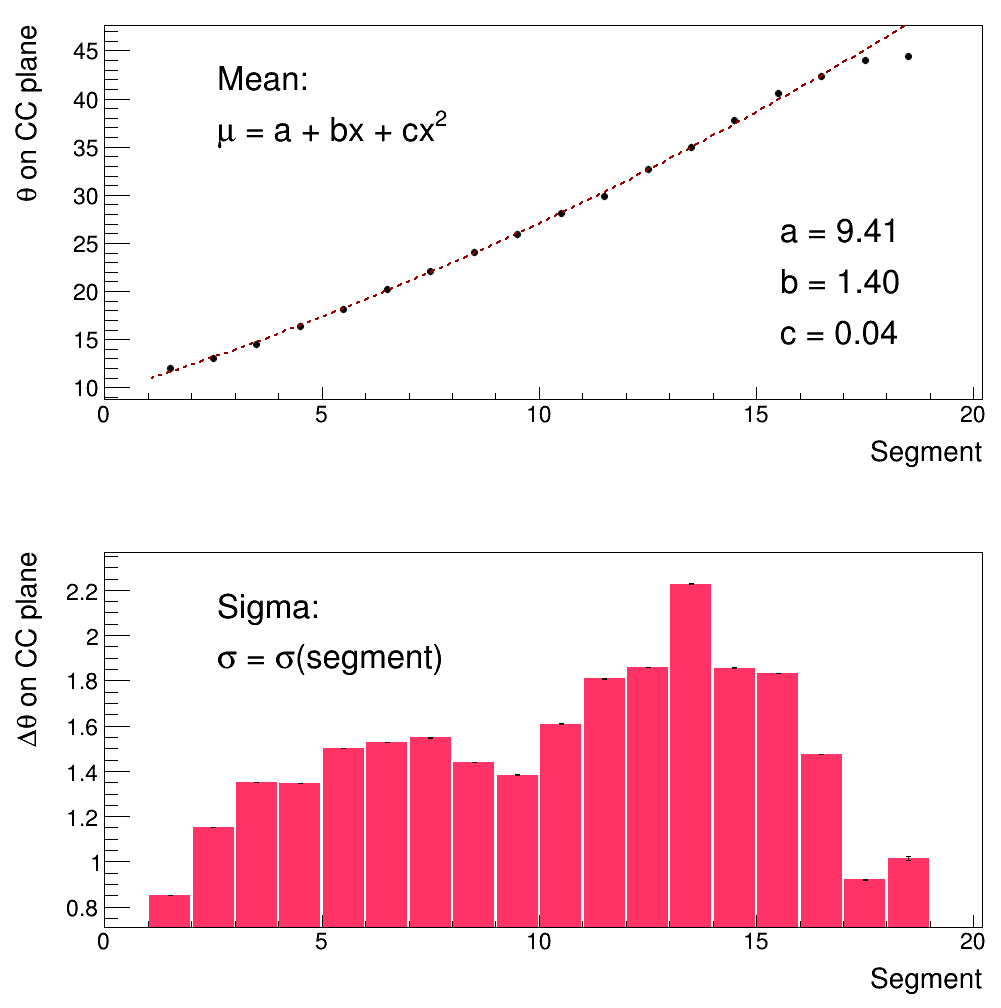
\includegraphics[width=0.88\textwidth]{img/cut-01-tmp_sector-1}
    \caption{Top panels: $\theta_{CC}$ for two segments in sector 1, and gaussian + second order
    polynomial fit. The distribution is slightly asymmetric to the
    left, so the lower limit was $4\sigma$ while the upper limit
    was $3\sigma$.
    Bottom Panels: the mean distribution is fitted with a third order
    polynomial.  }
    \label{fig:ccm_slices}
\end{figure}


\begin{figure}[ht]
    \centering
    \includegraphics[width=0.98\textwidth]{img/cut-01-tmc_sector-1}
    \caption{$\theta_{CC}$ versus Segment for Sector 1. The $\theta_{CC}$
        distribution for each segment is fitted with a gaussian +
        second order polynomial distribution to determine its mean
        and width. Events that have $\mu - 4\sigma < \theta_{CC} < \mu - 3\sigma$
        pass the cut.
        Top left: all events. Top right: events with calorimeter cuts applied
        (notice that these cuts remove $74 \,^{\circ\!\!}/\!_\circ$ of the data).
        Bottom left: events with the negative calorimeter cuts applied.
        Bottom right: all cuts applied. Notice that the CC matching cut
        only removes $7  \,^{\circ\!\!}/\!_\circ$ of the events with
        the calorimeter cuts already applied.}
    \label{fig:ccm_theta}
\end{figure}

\clearpage\newpage

\subsection{CC phi Matching}
The principle of this cut is very simple: when the track is on the right of the CC, the right
photo-multiplier should fire, and viceversa. Exception: when $\phi$ (relative to the center
in each sector) is less than $4^0$ the track is kept (the \v Cerenkov light should hit both
pmts, but with less efficiency since it splits in the middle)\cite{bib:ccmatch},\cite{bib:pc_fxpun}, \cite{bib:pc_osi}.

To show the effects of this cut the quantity ``$\phi$ matching'' is plotted in
Fig.~\ref{fig:ccm_phi}. This quantity is $0$ when both pmts are fired, $1(-1)$ when
there is a left (right) match and $2(-2)$ there is a left (right) mismatch.
The cut applied is: ``$\phi$ matching''$<2$ except when $|\phi|<4^0$.




\begin{figure}[ht]
    \centering
    \includegraphics[width=0.95\textwidth]{img/cut-02-pm_sector-1}
    \caption{``$\phi$ matching``: this quantity is $0$ when both pmts are fired, $1(-1)$ when
    there is a left (right) match and $2(-2)$ there is a left (right) mismatch.
    The cut applied is: ``$\phi$ matching''$<2$ except when $|\phi|<4^0$.}
    \label{fig:ccm_phi}
\end{figure}


\clearpage\newpage

\subsection{CC time Matching}\label{subsec:cc-time-matching}
The CC timing was not calibrated in e1-6, but a timing cut is still possible if applied to each tube
(this is basically equivalent to perform the timing calibration).

The difference $\Delta T$ between the track time recorded on a CC segment and corresponding time recorded on the TOF,
corrected for the path length from the CC to the TOF, is fitted with a gaussian (see Fig.~\ref{fig:cc_time_slices}).
Since there could be multiple \v Cerenkov light reflections leading to a time delay,
a 3 sigma cut is applied on the {\textit left} of the signal, and not on the right.
This difference is plotted in Fig.~\ref{fig:cc_time_sec1} for all tubes in sector one.

\begin{figure}[ht]
    \centering
    \includegraphics[width=0.46\textwidth]{img/slice-03_cut-03-tim_sector-1}
    \includegraphics[width=0.46\textwidth]{img/slice-08_cut-03-tim_sector-1}
    \includegraphics[width=0.46\textwidth]{img/slice-12_cut-03-tim_sector-1}
    \includegraphics[width=0.46\textwidth]{img/slice-15_cut-03-tim_sector-1}
    \caption{CC time matching. The difference $\Delta T$ between the track time recorded
    at a CC tube ($T_{CC}$) and corresponding time recorded on the TOF ($T_{SC}$),
        corrected for the path length from the CC to the TOF ($|\vec{R_{CC}}-\vec{R_{SC}}|/c$),
        shown here for 4 CC pmts, is fitted with a gaussian.
        A 5$\sigma$ cut is applied on the left of the signal.}
    \label{fig:cc_time_slices}
\end{figure}

\begin{figure}[ht]
    \centering
    \includegraphics[width=0.98\textwidth]{img/cut-03-timc_sector-1}
    \caption{CC time matching. The difference $\Delta T$ between the track time recorded
    at a CC tube ($T_{CC}$) and corresponding time recorded on the TOF ($T_{SC}$),
        corrected for the path length from the CC to the TOF ($|\vec{R_{CC}}-\vec{R_{SC}}|/c$),
        is fitted with a gaussian. A 3$\sigma$ cut is applied on the left of the signal.
        Top left: all events. Top right: events with calorimeter cuts applied.
        notice that these cuts remove $71 \,^{\circ\!\!}/\!_\circ$ of the data.
        Bottom left: events with the negative calorimeter cuts applied.
        Bottom right: all cuts applied. Notice that the CC matching cut
        only removes $7  \,^{\circ\!\!}/\!_\circ$ of the events with
        the calorimeter cuts already applied.}
    \label{fig:cc_time_sec1}
\end{figure}


%\clearpage\newpage
\subsection{EC Threshold}
A study \cite{bib:ecmin} of the inclusive cross section at various beam energies in CLAS 
results in a parametrization of the low momentum cut $p_{min}$ as a function of
the calorimeter low total threshold (in milliVolts) of the trigger discriminator:
\begin{equation}
 \label{eq:pmin} 
 p_{min}\,\,{\rm (MeV)} = 214 + 2.47\times EC_{threshold}{\rm (mV)}
\end{equation}

The low total threshold for e1-6 was $172$ mV therefore the minimum momentum cut is fixed at:
$$
p_{min} = 0.64\,\,{\rm GeV}
$$

Fig.~\ref{fig:pmincut_alls} shows for the momentum distribution of the candidates integrated
over all sectors. In average, $\sim 27.7\%$  pass the all other particle ID
cuts and of these, $91.9\%$ pass the minimum $p$ cut.

The cut value used is the same for all sectors and its effectiveness is summarized in 
table\,\ref{tab:pmincut}.


\begin{figure}[ht]
  \centering
		\includegraphics[width=0.88\textwidth]{img/cut-04-ec-threshold_sector-1.png}
		\caption{Candidates Momentum distribution in each sector. The minimum momentum cut is
               chosen according to Eq.\ref{eq:pmin}. In average, $\sim 82 \,^{\circ\!\!}/\!_\circ$ 
					of the candidates have a signal in the EC. Of those, $30 \,^{\circ\!\!}/\!_\circ$
					pass the all other particle ID cuts and of these, $92.5 \,^{\circ\!\!}/\!_\circ$
					pass the minimum $p$ cut.}
 		\label{fig:pmincut_alls}
\end{figure}

\clearpage



\begin{table}[h]
\label{tab:pmincut}
	\begin{center}
		\begin{tabular}{c | c | c | c}
			\hline 
			\multirow{2}{*}{Sector} 
					& all other cuts & minimum $p$ cut \\
					&  GeV & \% &  \\
			\hline 
			1   & 71.1 & 93.1 \\
			2   & 72.1 & 89.8 \\
			3   & 71.9 & 91.6 \\
			4   & 71.8 & 93.7 \\
			5   & 75.2 & 90.0 \\
			6   & 72.6 & 92.8 \\
			\hline
		\end{tabular}
		\caption{The minimum $p$ cut values and effectiveness in each sector.
					The last column refers to events with signal in EC that pass the 
 					minimum $p$ cut.}	
	
	\end{center}
\end{table}




\begin{thebibliography}{mybib}
    \bibitem{bib:ectotmax} {S. Stepanya},              {\textit Private Communication}
    \bibitem{bib:pc_osi}   {M. Osipenko},              {\textit Private Communication}
    \bibitem{bib:pc_fxpun} {F.X. Girod, P. Khetarpal}, {\textit Private Communication}
    \bibitem{bib:dc}       {M.D. Mestayer et al.}, The CLAS Drift Chamber System                 {\textit Nucl. Inst. and Meth. A 449, 81 (2000)}
    \bibitem{bib:ftof}     {E.S. Smith et al.},    The Time-of-Flight System for CLAS,           {\textit Nucl. Inst. and Meth. A 432, 265 (1999)}
    \bibitem{bib:ec}       {M. Amarian et al.},    The CLAS Forward Electromagnetic Calorimeter, {\textit Nucl. Inst. and Meth. A 460, 239 (2001).}
    \bibitem{bib:cc}       {G. Adams et al.},      The CLAS Cerenkov Detector,                   {\textit Nucl. Inst. and Meth. A 465, 414 (2001).}
    \bibitem{bib:ecmin}    {K.S. Egiyan},              \href{http://www.jlab.org/Hall-B/notes/clas_notes99/ec_thresh.ps}          {\textit CLAS NOTE 99 - 007}
    \bibitem{bib:ccmatch}                   {M. Osipenko, A. Vlassov and and M. Taiuti } \href{http://www1.jlab.org/ul/Physics/Hall-B/clas/public/2004-020.pdf}     {\textit CLAS NOTE 04 - 020}
    \bibitem{bib:pi0_resonance_id_electron} {M.Ungaro},                                  \href{https://maureeungaro.github.io/home/meson/pi0_resonance/electron_id} {\textit Electron identification for single $\pi^0$ elctroproduction in the first and second resonance regions}
\end{thebibliography}

\begin{thebibliography}{mybib}
    \bibitem{bib:ectotmax} {S. Stepanya},              {\textit Private Communication}
    \bibitem{bib:pc_osi}   {M. Osipenko},              {\textit Private Communication}
    \bibitem{bib:pc_fxpun} {F.X. Girod, P. Khetarpal}, {\textit Private Communication}
    \bibitem{bib:dc}       {M.D. Mestayer et al.}, The CLAS Drift Chamber System                 {\textit Nucl. Inst. and Meth. A 449, 81 (2000)}
    \bibitem{bib:ftof}     {E.S. Smith et al.},    The Time-of-Flight System for CLAS,           {\textit Nucl. Inst. and Meth. A 432, 265 (1999)}
    \bibitem{bib:ec}       {M. Amarian et al.},    The CLAS Forward Electromagnetic Calorimeter, {\textit Nucl. Inst. and Meth. A 460, 239 (2001).}
    \bibitem{bib:cc}       {G. Adams et al.},      The CLAS Cerenkov Detector,                   {\textit Nucl. Inst. and Meth. A 465, 414 (2001).}
    \bibitem{bib:ecmin}    {K.S. Egiyan},              \href{http://www.jlab.org/Hall-B/notes/clas_notes99/ec_thresh.ps}          {\textit CLAS NOTE 99 - 007}
    \bibitem{bib:ccmatch}                   {M. Osipenko, A. Vlassov and and M. Taiuti } \href{http://www1.jlab.org/ul/Physics/Hall-B/clas/public/2004-020.pdf}     {\textit CLAS NOTE 04 - 020}
    \bibitem{bib:pi0_resonance_id_electron} {M.Ungaro},                                  \href{https://maureeungaro.github.io/home/meson/pi0_resonance/electron_id} {\textit Electron identification for single $\pi^0$ elctroproduction in the first and second resonance regions}
\end{thebibliography}


\end{document}








